\chapter{مفاهيم اساسية}

سنتعرف في هذا الفصل على المعادلة بشكل عام وعلى انواع المعادلات ومن ثم نتعرف على النظام ومكونات النظام و نتطرق الى انظمة المعادلات سواء في متغير واحد او في $n$ من المتغيرات.

\section*{المعادلة الرياضية (1 - 1)\sen{\cite{odesolapp}}:}
هي عبارات رياضية تربط بينها علامة المساواة ويكون لها حدان متساويان في القيمة احدهما على الجانب الايمن والآخر على الجانب الايسر حيث يتم استخدامها في ايجاد المتغير المجهول سواء كان متغير واحد او اكثر.

\section*{المعادلة الجبرية (1- 2)\sen{\cite{odesolapp}}:}
هي مساواة بين مقدارين جبريين يحوي احدهما او كلاهما متغيراً او اكثر حيث القيمة العددية للمقدار الاول لا تساوي القيمة العددية للمقدار الثاني الا مع قيم خاصة للمتغيرات.\\
على سبيل المثال معادلة حدودية احادية المتغير تأخذ الشكل التالي
\[
a_n x^n + a_{n-1}x^{n-1} + \cdots + a_1 x + a_0 = 0
\]
حيث $a_0, \dots, a_n$ هي معاملات المعادلة، الهدف هو ايجاد جميع القيم المجهولة لــ $x$.

\begin{note}
	يقال عن متعددة الحدود انها من الدرجة الاولى اذا كانت اعلى قوة لــ $x$ تظهر في المعادلة هي واحد. وانها من الدرجة الثانية اذا كانت اعلى قوة لــ $x$ هي 2 وهكذا ...
\end{note}

\section*{المعادلة التفاضلية (1 - 3)\sen{\cite{odesolapp}}:}
هي معادلة تحوي مشتقات و تفاضلات لبعض الدوال الرياضية وتظهر فيها بشكل متغيرات المعادلة ويكون الهدف من حل هذه المعادلات هو ايجاد هذه الدوال الرياضية التي تحقق مشتقاتها هذه المعادلات.\\
\\
\textbf{$\bullet$ درجة المعادلة الرياضية :}
تتحدد درجة المعادلة التفاضلية حسب اس المشتقة ذات الرتبة الاعلى.\\ \\
\textbf{$\bullet$ رتبة المعادلة التفاضلية :}
هي رتبة اعلى مشتقة تحتوي عليها هذه المعادلة.\\
\noindent
\textbf{مثال:}
	\begin{table}[H]
		\renewcommand{\arraystretch}{1.4}
		\centering
		\begin{tabular}{|c|c|c|}
			\hline
			\textbf{المعادلة التفاضلية} & \textbf{الدرجة} & \textbf{الرتبة}\\
			\hline
			$(y')^2 + 5x^3 y = 2x + 5y$ & الثانية & الاولى\\
			\hline
		\end{tabular}
	\end{table}

\section[انواع المعادلات التفاضلية]{انواع المعادلات التفاضلية}

\begin{enumerate}
\item \textbf{معادلات تفاضلية اعتيادية (\en{ordinary differential equations})} تحتوي على توابع ذات متغير مستقل واحد ومشتقات هذا المتغير \\
\textbf{مثال}:\qquad $y'' + 3y = x^2$
\item \textbf{معادلات تفاضلية جزئية \en{partial differential equations}} هي معادلات تفاضلية تحتوي على دالة واحدة او اكثر من الدوال المجهولة ومشتقاتها الجزئية.\\
\textbf{مثال:}\[
\frac{\partial u}{\partial x} + 3 \frac{\partial u}{\partial y} = 0
\]
\end{enumerate}

\section{بعض طرق حل المعادلات التفاضلية الجزئية}
\begin{enumerate}[label=$\bullet$]
	\item \textbf{فصل المتغيرات:}\\ بهذه الطريقة يتم تحويل المعادلة التفاضلية الجزئية ذات $n$ من المتغيرات المستقلة الى معادلة تفاضلية اعتيادية.
	
	\item \textbf{التحويلات التكاملية:}\\ يتم تحويل المعادلة الجزئية ذات $n$ من المتغيرات المستقلة الى معادلة تفاضلية جزئية ذات $n-1$ من المتغيرات المستقلة ومن ثم بهذه الطريقة يمكن تحويل المعادلة الجزئية ذات المتغيرين الى معادلة اعتيادية.
	
	\item \textbf{طريقة الدوال الذاتية: }\\ يتم ايجاد حل المعادلة الجزئية كمجموع عدد غير منته من الدوال الذاتية وهذه الدوال توجد بحل يسمى المناظرة للمسائل الاصلية.
\end{enumerate}

\section*{المعادلات التفاضلية الخطية وغير الخطية (1 - 4)}

كل من المعادلات التفاضلية العادية و الجزئية يمكن ان تصنف الى خطية وغير خطية وتكون المعادلة التفاضلية خطية بشرطين:
\begin{enumerate}[label=\textcolor{red}{$\bullet$}]
	\item اذا كانت معاملات المتغير التابع والمشتقات فيها دوال في المتغير المستقل فقط او ثوابت.
	
	\item اذا كان المتغير التابع والمشتقات غير مرفوعة لأسس اي كلها من الدرجة الاولى.
\end{enumerate}  
\noindent
$\bullet$ وتكون غير خطية فيها عدا ذلك
\\[10pt]
كل معادلة تفاضلية خطية هي من الدرجة الاولى بينما ليست كل المعادلات التفاضلية من الدرجة الاولى هي خطية لان الدرجة تتحدد حسب اس التفاضل الاعلى ومن الممكن ان تكون التفاضلات الاقل مرفوعة لأسس غير الواحد دون ان يؤثر ذلك على الدرجة وهذا يخل بشرط المعادلة الخطية. وبهذا تكون غير خطية.
\\[10pt]
\noindent
\textbf{امثلة:}
\begin{enumerate}
	\item $x^2 y'' + xy' + x^2 y = e^x \sin x$\qquad معادلة تفاضلية خطية.
	\item $yy'' + y' = x$\qquad\qquad\qquad\quad معادلة تفاضلية غير خطية.
\end{enumerate}
\section*{النظام الخطي (1 - 5)\sen{\cite{odesolapp}}:}
هو نظام مكون من $m$ من المعادلات و $n$ من المتغيرات. او هو مجموعة تحتوي $m$ من المعادلات الخطية لكل منها $n$ من المتغيرات ويعبر عن ذلك النظام عادة بالشكل
\renewcommand{\theequation}{\arabic{chapter}-\arabic{equation}}
\begin{equation}
	\begin{gathered}
	a_{11}x_1 + a_{12}x_2 + \cdots + a_{1n} x_n = b_1\\
	a_{21}x_1 + a_{22}x_2 + \cdots + a_{2n} x_n = b_2\\
\vdots\\
	a_{m1}x_1 + a_{m2}x_2 + \cdots + a_{mn} x_n = b_m
\end{gathered}
\end{equation}
\\ \\
بالتالي فإن المعادلة (1-1) هي $a_{i1}x_1+a_{i2}x_2 +\cdots+a_{in}x_n=b_i$. تسمى $a_{ij}$ بالثوابت. تسمى $S_i$ التي تحقق كل معادلة خطية في النظام اعلاه بحل النظام المعادلات الخطية
\[
a_1x_1 + a_2 + \cdots + a_n x_n = b
\]

\section*{حل المعادلة الخطية (1 - 6)\sen{\cite{odesolapp}}:}
هو متتابعة من $n$ من الاعداد $S_1,S_2,\dots,S_n$ تحقق المعادلة عند اجراء التعويض وتسمى الفئة المكونة من كل  حلول المعادلة بفئة الحل لها.

\section*{انظمة المعادلات الخطية في متغيرين (1 - 7)\sen{\cite{research}}:}
هذا النظام يكون بالشكل
\begin{gather*}
	A_1 X_1 + B_1X_2 = C_1\\
	A_2 X_1 + B_2 X_2 = C_2
\end{gather*}
حل هذا النظام هو مجموعة الازواج المرتبة من الاعداد الحقيقية والتي تحقق المعادلتين. سوف نستخدم طريقة الحذف والتعويض الخلفي لحل هذا النظام.\\
\\
\noindent
\textbf{مثال}
\\ \noindent
	اوجد حل النظام
	\begin{gather}
		3X - 4Y = 28\\
		X+2Y = 6
	\end{gather}
	\noindent
	\textbf{الحل}\\
	\noindent
	من المعادلة (1-3)
	\begin{equation}
		X = 6 -2Y
	\end{equation}
	نعوض (1-4) في (1-2)
	\begin{gather*}
		3(6-2Y) - 4Y = 28\\
		18 - 6Y - 4Y = 28\\
		-10 Y = 10\\
		\Rightarrow Y = -1
	\end{gather*}
	نعوض في (1-4)
	\[
	X = 6-2(-1) = 6+2 = 8
	\] 
	النظام يمتلك حل وحيد.

\section*{انظمة المعادلات في ثلاث متغيرات (1 - 8)\sen{\cite{odesolapp}}:}
تكون بالشكل
\begin{gather*}
	a_1 x + b_1 y + c_1 z = d_1\\
	a_2 x + b_2 y + c_2 z = d_2\\
	a_3 x + b_3 y + c_3 z = d_3
\end{gather*}
\noindent
\textbf{مثال}\\ \noindent
	حل النظام
	\begin{gather}
		2x + 2y - 3z = 1\\
	5x + 3y - 4z = 4 \\
	7x - 3y + 2z =6
	\end{gather}
	
	\noindent
	\textbf{الحل}\\
	\noindent
	يكون الحل بطريقة الحذف. نضرب المعادلة (1-5) بــ $-3$ و المعادلة (1-6) بــ 2
	نحصل على 
	\begin{gather}
		-6x -6y +9z =-3\\
		10x + 6y -8z =8
	\end{gather}
	بجمع (1-8) و (1-9) نحصل على 
	\begin{equation}
		4x + z =5
	\end{equation}
	الآن نجمع (1-6) مع (1-7) نحصل على
	\begin{equation}
		12x -2z = 10 \Rightarrow 6x - z = 5  
	\end{equation}
	بجمع (1-10) و (1-11) نحصل على
	\[
	10x = 10 \Rightarrow x=1
	\]
	نعوض في (1-10)
	\[
	4(1) + z = 5 \Rightarrow z=1
	\]
	نعوض الآن عن $x, z$ في (1-5)
	\[
	2(1) + 2y - 3(1) = 1 \Rightarrow y =1
	\]
	نتحقق من ان  $x=1, y=1,z=1$ يحقق حل النظام.
	\begin{gather*}
		2(1) + 2(1)- 3(1) =1\\
		5(1)+3(1)-4(1)=1\\
		7(1)-3(1)+2(1)=1
	\end{gather*}

\section[المعنى الهندسي للنظام الخطي]{المعنى الهندسي للنظام الخطي\sen{\cite{odesolapp}}:}
النظام الخطي العام المتكون من معادلتين خطيتين بالمتغيرين $x,y$ يمثل بالصيغة التالية
\begin{gather*}
	a_1x + b_1 y = c_1\\
	a_2 + b_2 y = c_2
\end{gather*}
ان الشكل الهندسي لهذه المعادلات هو الخطوط المستقيمة $L_1, L_2$ كما في الشكل (1 - 1)
ولما كانت النقطة $(x, y)$ تقع على المستقيم اذا وفقط اذا كانت $x, y$ تحقق معادلة المستقيم فإن حلول النظام الخطي تقابل المستقيمين كما موضح في الشكل (1 - 1)
\begin{figure}[H]
	\centering
	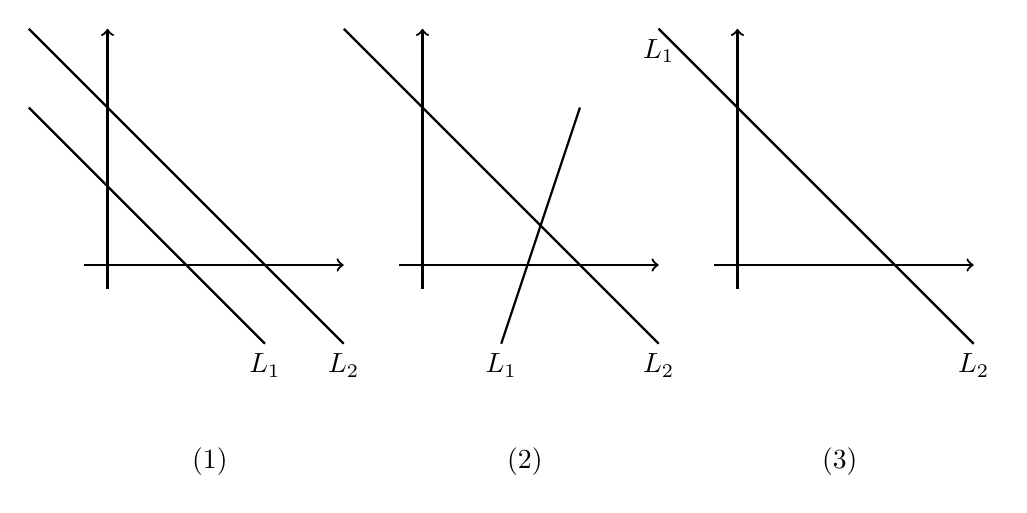
\begin{tikzpicture}
		\node at (1.3, -2.5) {(1)};
		\draw[->, thick] (-0.3,0) -- (3, 0);
		\draw[->, thick] (0, -0.3) -- (0, 3);
		
		\draw[thick] (-1, 2) -- (2, -1) node[below]{$L_1$};
		\draw[thick] (-1, 3) -- (3, -1) node[below]{$L_2$};
		
				\node at (5.3, -2.5) {(2)};
\draw[->, thick] (3.7,0) -- (7, 0);
\draw[->, thick] (4, -0.3) -- (4, 3);

\draw[thick] (6, 2) -- (5, -1) node[below]{$L_1$};
\draw[thick] (3, 3) -- (7, -1) node[below]{$L_2$};

		\node at (9.3, -2.5) {(3)};
\draw[->, thick] (7.7,0) -- (11, 0);
\draw[->, thick] (8, -0.3) -- (8, 3);

\draw[thick] (7, 3) -- (11, -1) node[pos=0, below]{$L_1$};
\draw[thick] (7, 3) -- (11, -1) node[below]{$L_2$};
	\end{tikzpicture}
\end{figure}
\begin{center}
	الشكل (1-1)
\end{center}
من خلال الشكل (1-1) يتضح ان هناك ثلاث احتمالات للحلول هي
\begin{enumerate}
	\item المستقيمان متوازيان اي لا يوجد نقطة تقاطع وعليه فليس للنظام الخطي حل (الشكل (1) من (1-1)).
	\item يتقاطعان بنقطة واحدة وهذا يعني ان النظام الخطي له حل واحد فقط. (الشكل (2) من (1-1)).
	\item المستقيمان متطابقان اي يوجد عدد غير محدد من الحلول (الشكل (3) من (1-1)).
\end{enumerate}
\noindent
\\
نستنتج من ذلك ان اي نظام خطي اما ليس له حل او له حل وحيد او له عدد غير منته من الحلول. تسمى المجموعة المنتهية من $m$ من المعادلات الخطية التي تحتوي على $n$ من المتغيرات 
$X_1, X_2 , \dots, X_n$
بنظام من المعادلات الخطية.\\ 
\noindent
وتسمى ايضاً بالنظام الخطي اما المتتابعة المتكونة من $n$ من الاعداد الحقيقية $S_1 , S_2, \dots, S_n=X_n$ حلاً لكل معادلة من النظام الخطي.\\
\noindent
ويمكن كتابة النظام الخطي من $m$ من المعادلات التي تحتوي على $n$ من المتغيرات بالصيغة
\begin{equation*}
	\begin{gathered}
		a_{11}X_1 + a_{12}X_2 + \cdots + a_{1n} X_n = b_1\\
		a_{21}X_1 + a_{22}X_2 + \cdots + a_{2n} X_n = b_2\\
		\vdots\\
		a_{m1}X_1 + a_{m2}X_2 + \cdots + a_{mn} X_n = b_m
	\end{gathered}
\end{equation*}
حيث $X_1 , X_2, \dots,X_n$ متغيرات و $a_{ij}$ ثوابت حيث 
$i=1,2,\dots,m, j=1,2,\dots,n$

\noindent
يعتبر وضع الدليلين لمعادلة المجاهيل وسيلة مقيدة نستخدمها لتحديد موضع المعامل في النظام. يشير الدليل الايسر للمعامل توجد $a_{ij}$ الى المعادلة التي تقع فيها المعامل ويشير الدليل الايمن الى المجهول المضروب فيه. ولهذا فإن $a_{n2}$ في المعادلة الاولى تضرب في المجهول $x_2$ يمكننا كتابة النظام الخطي على الشكل
\[
\left(
\begin{array}{cccc|c}
	a_{11} & a_{12} & \cdots & a_{1n} & b_1\\
	a_{21} & a_{22} & \cdots & a_{2n} & b_2\\
	\vdots&\vdots&\ddots&\vdots &\vdots\\
	a_{m1} & a_{m2} & \cdots& a_{mn} & b_m
\end{array}
\right)
\]
ويسمى هذا الترتيب بالمصفوفة الممتدة للنظام.\\
مستطيل من الاعداد وتظهر المصفوفات فيه. ويستخدم لفظ مصفوفة في الرياضيات ليدل على ترتيب مقامات عديدة.\\
\noindent
 لتوضيح ان المصفوفة الممتدة لنظام المعادلات.
 \begin{gather*}
 	X + 2Y + 2Z = 4\\
 	X+Y +4Z = 6\\
 	2X - 6Y - 2Z =-2
 \end{gather*}
 هي
 \[
 \left(
 \begin{array}{ccc|c}
 	1&2&2&4\\
 	1&1&4&6\\
 	2 &-6& -2& -2
 \end{array}
 \right)
 \]
 \noindent
\textbf{ملاحظة:}\\ \noindent
 	عند بناء اي مصفوفة ممتدة يجب كتابة المجاهيل بنفس الترتيب في كل معادلة.
 	الطريقة الاساسية لحل جديد له نفس الحل ولكن ابسط في الحل اي نظام لمعادلات خطية هي النظام المعطى بنظام يتم الحصول بشكل عام على النظام الجديد من سلسلة من الخطوات بواسطة تطبيق الانواع الثلاثة الآتية من عمليات حذف منتظم من المجاهيل.
 \begin{enumerate}
 	\item ضرب المعادلة بأكملها بثابت غير صفري.
 	\item التبديل بين  اي معادلتين.
 	\item اضافة مضاعف لصف آخر.
 \end{enumerate}  
  تسمى هذه العمليات بعمليات اولية على المصفوفة. سنوضح في المثال التالي كيفية استخدام هذه العمليات.

\noindent \textbf{مثال:} \\ \noindent
حل النظام الخطي
\begin{gather*}
	X-2Y + 3Z=9\\
	-X +3Y =-4\\
	2X-5Y+5Z=17
\end{gather*}
\textbf{الحل:}\\
1. المصفوفة الممتدة للنظام
 \[
\left(
\begin{array}{ccc|c}
	1&-2&3&9\\
	-1&3&0&-4\\
	2 &-5& 5& 17
\end{array}
\right)
\]
2. نجمع الصف الاول مع الصف الثاني. ونضرب الصف الاول بــ $-2$ ونجمعها مع الصف الثالث نحصل على
 \[
\left(
\begin{array}{ccc|c}
	1&-2&3&9\\
	0&1&3&5\\
	0 &-1& -1& -1
\end{array}
\right)
\]
3. نجمع الصف الثاني والثالث نحصل على
 \[
\left(
\begin{array}{ccc|c}
	1&-2&3&9\\
	0&1&3&5\\
	0 &0& 2& 4
\end{array}
\right)
\]
اي نحصل على
\begin{align}
	X-2Y+3Z&=9\\
	Y + 3Z=5\\
	2Z=4
\end{align}
من معادلة (1-14) نحصل على 
\[
Z=2
\]
نعوض في (1-13) نحصل على 
\[
Y + 3(2) = 5 \Rightarrow Y = -1
\]
الآن نعوض في (1-12) نحصل على
\[
X - 2(-1) + 3(2) = 9 \Rightarrow X = 1
\]